\chapter{Conclusion}
\label{chap:conclusion}

\section{General Contributions}

The work presented in this thesis deals with planning optimal motions
for anthropomorphic systems in general, and humanoid robots in
particular. Based on promising but still separate advances in motion
planning and optimization in high-dimensional spaces, the main focus
of this work was set on the combination of methods from both fields in
order to generate optimal collision-free trajectories for humanoid
robots.

More precisely, the contributions lead to the development of :
\begin{itemize}
\item an efficient A$^*$-based path optimization algorithm for a
  bounding-box representation of a humanoid robot. It was inserted in
  an existing two-stage planner which allowed the generation of
  minimum-time dynamic walking trajectories.
\item a whole-body motion planner for humanoid robots. Based on the
  small-space controllability property which was established in this
  work, collision-free trajectories that seamlessly combine dynamic
  walking and manipulation were produced.
\item a two-stage optimal motion planning framework which combines
  constrained sampling-based planners with optimal control
  methods. Dynamically-feasible collision-free smooth trajectories
  were successfully generated in constrained environments.
\end{itemize}

Finally, special care was given in this thesis to generate feasible
motions that not only can be executed on digital actors, but also on
physical humanoid robots in real environments. Therefore, resulting
motions from all previously cited contributions were successfully
executed on the HRP-2 humanoid robot.

\section{Perspectives}

Let us recall that planning represents only one of the three
components of the perception-planning-action paradigm. We want
humanoid robots to achieve tasks such as locomotion in a reactive way;
it is therefore obvious that the time which is spent in the planning
component should be very short, i.e.\ motions should be generated very
quickly. This work succeeded in the development of generic methods for
planning optimal motion for humanoid robots, but their computational
efficiency remains one of their main limitations, as computation time
was not the focus of this work. Some pointers were thus given in the
previous chapter discussions in order to address this issue.

Humanoid robots have formidable abilities when compared to more common
fixed-base or wheeled robots: thanks to their legged structure, they
can walk, step over obstacles, run, climb hills and execute acrobatic
figures among many things. This thesis was limited to generating
motions where a humanoid robot is standing on a flat horizontal floor;
this voluntary limitation allowed us to devise sound methods for
whole-body dynamic walking and optimal motion planning. Nevertheless,
insights for extending our optimal motion planning framework to handle
a set of non-coplanar contact points were given.

\bigskip

In some sense, both the computer graphics community and the robotics
one share the common goal of generating feasible motions, with the
former's main concern being the motion realism with respect to the
laws of Physics, and the latter's being its feasibility on complex
hardware platforms in the physical world. Thanks to a smart usage of
online model-predictive control techniques for digital avatar
animation \cite{coros2010generalized,tassa2012synthesis}, recent
results have shown that we can hope to make humanoid robots plan
extreme locomotion reactively. However, beside a transcription of the
above algorithms to humanoid robots, we need to make sure that we have
both the right hardware and control software.

Consider for instance a back-flip motion, as shown in Figure
\ref{fig:chap4-romeo-back-flip}. The robot must first exert adequate
forces on the floor to jump in the air, rotate during the flying
phase, then land back on its feet. Most mainstream humanoid robots,
such as the HRP-2, are capable of pushing sufficiently to jump in the
air, but their actuators are such that they cannot quickly transform
the kinetic energy acquired in the flying phase into other energies
when they hit the ground; this energy is thus entirely transmitted to
the mechanical structure and might cause it to break. Introducing
backdrivable actuators in the robot structure can help addressing this
issue by allowing the fast transformation of the kinetic energy back
into electric energy and keeping the physical system
integrity. Furthermore, the generated current measurements can give a
good idea of the actuator torques, which paves the way for the
implementation of force-based control laws. Such laws, compared with
position-based control laws, can be extremely useful in retaining the
robot balance during fast motions.

\bigskip

In light of these results, we would like to tackle, in our future
works, the themes of model-predictive control and stabilization for
force-controlled humanoid robots.

\begin{figure}
  \centering
      {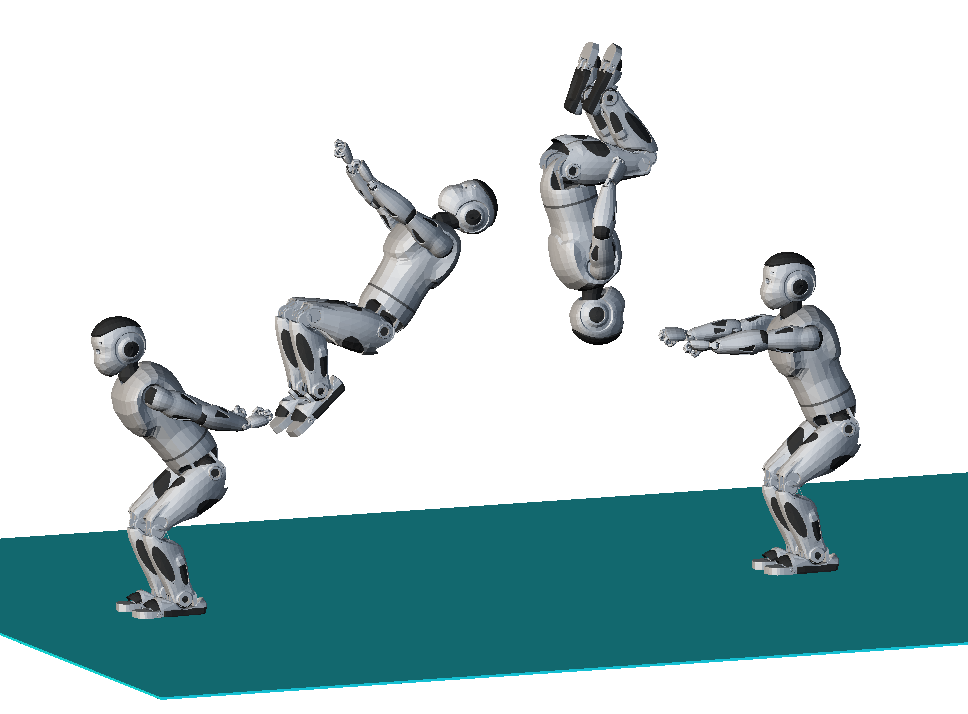
\includegraphics[width = 0.8\linewidth]
        {src/chap4-conclusion/romeo-back-flip.png}}
      \caption{A humanoid robot executes a back-flip. This is a highly
        dynamic motion where the flying phase is difficult to control,
        and the foot forces on impact may be high.}
      \label{fig:chap4-romeo-back-flip}
\end{figure}
